\documentclass{projetofinal-dcc}

%%%%%%%%%%%%%%%%%%%%%%%%%%%%%%%%%%%%%%%%%%%%%%%%%%%%%%%%%%%%
%I N I C I O  D O  D O C U M E N T O
%%%%%%%%%%%%%%%%%%%%%%%%%%%%%%%%%%%%%%%%%%%%%%%%%%%%%%%%%%%%
\begin{document}

\title{Análises do transporte público rodoviário no Rio de Janeiro através de Dados Abertos}

\author{Mário Alberto Cecchi Raduan}{Ao longo da minha graduação, tive o privilégio de conhecer e trabalhar com diversas pessoas que foram essenciais para que eu chegasse até aqui.

Apesar das dificuldades passadas pela Universidade durante esses anos, incluindo duas longas greves, pude contar com a ajuda de excelentes profissionais que me ajudaram ao longo desse caminho. Entre eles, agradeço imensamente ao mestre Adriano J. O. Cruz, por ter me apresentado ao mundo da pesquisa através de duas iniciações científicas - que me envolveram muito mais na Universidade do que eu podia esperar - e por ter me ensinado tanto de Computação. Agradeço também à professora Valeria Menezes Bastos, por ter sido uma excelente professora e orientadora, e que me motivou tanto durante a reta final da minha graduação.

Agradeço a todo o pessoal do LabIC - Laboratório de Inteligência Computacional - que me acolheu durante a maior parte da graduação, não só como um laboratório, como também um refúgio pessoal e um lugar de muitas amizades.

Agradeço à minha família - meu pai, José Raduan, minha mãe, Ana Elisa Cecchi, minha irmã, Daniela Cecchi, meu irmão, Giancarlo Raduan e meu avô, Mario Fernando Cecchi - por todo o apoio dado durante esses anos. Vocês foram incríveis e me motivaram para que eu chegasse até aqui, sempre pensando na minha educação, minha felicidade e meu futuro.

Agradeço a todo o pessoal do Rio Bus, especialmente ao Fred Souza e Marquinho Tormenta, com quem aprendi muito e serviu como inspiração para este projeto final.

Agradeço aos meus amigos - da turma do BCC de 2011.1, do LabIC, de Glasgow e da Ilha - por terem me mantido são durante a faculdade, mesmo nas horas em que isso parecia impossível. Agradeço também ao Danilo Vettorazzi, que além de ter sido um grande amigo durante toda a faculdade, me ajudou a escolher o tema deste projeto final e pediu para que eu colocasse o nome dele aqui.

Por fim, agradeço ao meu namorado, Marcos Moretto, por ter sido um ótimo companheiro e, principalmente, amigo durante os últimos anos. Você foi essencial em todos os aspectos.
}

\advisor[Profa.]{Valeria Menezes Bastos,~D.Sc.}{}


\banca[Profa.]{Adriana Santarosa Vivacqua,~D.Sc.}{DCC~-~UFRJ}
\banca[Prof.]{Vinícius Gusmão Pereira de Sá,~D.Sc.}{DCC~-~UFRJ}

\location{Rio~de~Janeiro}{RJ}{Brasil}

% mês e ano de defesa
\date{Novembro}{2016}
\maketitle

\startdocument
%%%%%%%%%%%%%%%%%%%%%%%%%%%%%%%%%%%%%%%%%%%%%%%%%%%%%%%%%%%%
%A G R A D E C I M E N T O S
%%%%%%%%%%%%%%%%%%%%%%%%%%%%%%%%%%%%%%%%%%%%%%%%%%%%%%%%%%%% 
\makethankspage

%%%%%%%%%%%%%%%%%%%%%%%%%%%%%%%%%%%%%%%%%%%%%%%%%%%%%%%%%%%%
%R E S U M O
%%%%%%%%%%%%%%%%%%%%%%%%%%%%%%%%%%%%%%%%%%%%%%%%%%%%%%%%%%%%
\begin{abstract}{
  Em tempos onde diversos dados governamentais passam a ser disponibilizados de maneira transparente para o público, começam a surgir diversas soluções de terceiros que fazem uso desses dados para auxiliar a população. Esses, agora processados e analisados, tornam-se ferramentas de informação nas mãos do cidadão e promovem a fiscalização dos serviços públicos prestados.

O escopo deste trabalho é baseado nos dados abertos da frota de ônibus da cidade do Rio de Janeiro, um dado fornecido pela Prefeitura carioca e que diz respeito às linhas municipais e à geolocalização de todos os ônibus em tempo real. Utilizaremos esses dados para elaborar algoritmos que permitem analisar o real funcionamento dos ônibus do Rio. Tais algoritmos colhem estatísticas que podem servir como um documento para a fiscalização desse serviço público tão essencial.

}
\end{abstract}

%%%%%%%%%%%%%%%%%%%%%%%%%%%%%%%%%%%%%%%%%%%%%%%%%%%%%%%%%%%%
%A B S T R A C T
%%%%%%%%%%%%%%%%%%%%%%%%%%%%%%%%%%%%%%%%%%%%%%%%%%%%%%%%%%%%
\begin{englishabstract}{
  In times where all kinds of governamental data become available in a transparent manner to the public, different third-party solutions arise making use of this data to help people. That data, now processed and analyzed, become information tools on the citizen's hands and promote the fiscalization of public services.

The studies presented in this document are based on the open data of Rio de Janeiro's city buses, made available by Rio's city hall, composed of information about the municipal bus lines and the geolocalization of all of their buses in real-time. We'll gather data to elaborate algorithms that allow the analysis of the real functioning of Rio's buses. Those algorithms gather statistics that can be used to promote the accountability of such an essential public service.
}
\end{englishabstract}

%%%%%%%%%%%%%%%%%%%%%%%%%%%%%%%%%%%%%%%%%%%%%%%%%%%%%%%%%%%%
%L I S T A S
%%%%%%%%%%%%%%%%%%%%%%%%%%%%%%%%%%%%%%%%%%%%%%%%%%%%%%%%%%%%
% Figuras
\makefigurespage

% Tabelas
\maketablespage

% Algoritmos
%\makelistingspage

% Abreviaturas (devem estar em ordem alfabética)
\makeabrevpage{\item [API] Application Programming Interface
\item [CSV] Comma-separated values
\item [DAG] Dados abertos governamentais
\item [FETRANSPOR] Federação das Empresas de Transporte de Passageiros do Estado do Rio de Janeiro
\item [GPS] Global Positioning System
\item [JSON] JavaScript Object Notation
\item [OD] Open Definition
\item [UFRJ] Universidade Federal do Rio de Janeiro
\item [URI] Uniform Resource Identifier
\item [URL] Uniform Resource Locator}

% Símbolos (devem estar em ordem alfabética)
%\makesymbolspage{\input{elementos-pretextuais/simbolos}}

% Sumário 
\maketocpage

%%%%%%%%%%%%%%%%%%%%%%%%%%%%%%%%%%%%%%%%%%%%%%%%%%%%%%%%%%%%
%C O N T E Ú D O
%%%%%%%%%%%%%%%%%%%%%%%%%%%%%%%%%%%%%%%%%%%%%%%%%%%%%%%%%%%%
\startcontent

\chapter{Introdução}\label{chp:CAP_INTRO}

Nos últimos anos, vivemos um momento de crescente participação popular na política brasileira. Com a crescente demanda por transparência na gestão pública, os governos assumem o compromisso de tornar públicos, através da internet, os dados de suas gestões - como arrecadações, gastos, licitações e dados de serviços públicos. Surge então um meio capaz de diminuir as barreiras para que a população fiscalize a atuação dos nossos representantes.

Entre os compromissos da transparência, está a disponibilização de dados abertos governamentais (DAGs), que consiste na distribuição de qualquer tipo de dado em posse do poder público em formatos que permitem qualquer cidadão consultar, analisar, se apropriar e redistribuí-los de maneira livre. Esses dados permitem não só uma maior fiscalização da administração pública, como também permitem que indivíduos e organizações possam utilizá-los para construir ferramentas de valor à sociedade.

No município do Rio de Janeiro, entre os diversos dados abertos oferecidos, estão os dados de transporte e mobilidade, que incluem informações sobre linhas de ônibus, metrô, trem, bicicletários e ocorrências de trânsito. Neste trabalho, serão utilizados os dados disponibilizados das linhas de ônibus municipais, que incluem informações dos GPS dos ônibus, a fim de observar o comportamento desses veículos e analisar o funcionamento desse serviço público na cidade.


\section{Objetivos}\label{sec:CAP_INTRO_OBJETIVOS}

O objetivo deste trabalho é elaborar uma ferramenta para o cidadão carioca poder fiscalizar a qualidade de serviço do transporte público rodoviário da sua cidade, através da análise dos dados reais obtidos pelos DAGs locais. Tal ferramenta permite ao usuário acessar relatórios diversos para auxiliar na compreensão desse serviço público prestado. Este trabalho foca no desenvolvimento de duas análises específicas: a densidade de ônibus por região e a frequência média dos ônibus de cada linha. 

A primeira análise foi selecionada devido à uma reflexão dos cariocas: "Por que há lugares que possuem tantos ônibus e outros que não são atendidos por nenhuma linha?". O estudo proposto serve para expor esse grande contraste e desigualdade presentes na cidade.

Já a segunda análise foi inspirada por uma das maiores dúvidas de qualquer usuário de ônibus: "Quanto tempo vai demorar para o meu ônibus chegar?". Para ajudar a responder esta pergunta, calcularemos os intervalos entre cada ônibus ao longo de um período, comprovando qual é o tempo médio de espera por cada linha. 

%Além disso, para tornar-se viável o segundo estudo, foi desenvolvido um algoritmo capaz de identificar o sentido (ida ou volta) dos ônibus. Tal algoritmo também será apresentado neste trabalho


\section{Motivação}\label{sec:CAP_INTRO_MOTIVACAO}

A ideia para este trabalho surgiu durante minha participação no Rio Bus\cite{riobus_sc} - um aplicativo móvel desenvolvido na Universidade Federal do Rio de Janeiro que utiliza DAGs para informar a localização dos ônibus de cada linha do Rio de Janeiro, servindo como grande utilitário para o usuário de ônibus carioca.

Esses usuários, muitas vezes por engano, enviavam para nós reclamações sobre o serviço dos ônibus - algo sobre o qual não temos responsabilidade. No entanto, pensamos em uma maneira de ajudar: fornecendo ao usuário relatórios de funcionamento dos ônibus e munindo-o com informações concretas para que possa enviar suas reclamações aos órgãos fiscalizadores.

Em paralelo, também houve uma procura pelos dados dos ônibus armazenados no Rio Bus por políticos que promoviam a CPI dos Ônibus\cite{cpi_dos_onibus}. Estes buscavam uma fonte alternativa aos burocráticos processos legais que fosse capaz de fornecer relatórios como evidência do descumprimento dos contratos por parte das concessionárias que operam as linhas de ônibus. Este foi um dos diversos pontos questionados na CPI, buscando apurar a eficácia dos instrumentos de controle das metas estabelecidas nos contratos com essas empresas.

Assim, graças ao transporte público extremamente deficiente do Rio de Janeiro e essa demanda por informação - que, idealmente, deveria ser pública - decidi desenvolver este projeto para tentar contribuir, de alguma maneira, com a melhoria desse essencial serviço. 

Ainda que não esteja em minhas mãos garantir que os usuários irão fazer uso desses dados para reivindicar seus direitos - e muito menos garantir que essas melhorias serão feitas - gostaria de contribuir com ferramentas que possam auxiliar isso. Além disso, todos os estudos e algoritmos desenvolvidos durante este projeto são \textit{open-source}, ou seja, de domínio público\footnote{"Código aberto, ou open source em inglês, é um modelo de desenvolvimento que promove um licenciamento livre para o design ou esquematização de um produto, e a redistribuição universal desse design ou esquema, dando a possibilidade para que qualquer um consulte, examine ou modifique o produto", de acordo com \cite{REF_OPEN_SOURCE}.}.


\section{Trabalhos relacionados}\label{sec:CAP_INTRO_TRABALHOS_RELACIONADOS}

Trabalhos anteriores buscaram analisar a definição e os impactos dos dados abertos na sociedade. Em \cite{REF_OGD_AND_IMPACT}, o autor descreve os fundamentos dos DAGs em quatro interpretações - como um direito, como movimento e como política - e analisa os impactos causados na \textit{accountability}, na melhoria dos serviços públicos e no crescimento econômico. Em \cite{REF_MONO_BUUS}, o autor traz um estudo de caso do Buus, uma empresa do Rio de Janeiro que faz uso dos mesmos DAGs que utilizaremos e que acompanhou o processo de abertura dos dados pela Prefeitura do Rio. São estudadas na prática as dificuldades e consequências dos usos desses dados, assim como diferentes modelos de negócios testados durante o desenvolvimento.

O próprio Google também possui ferramentas que fazem uso dos DAGs do Rio de Janeiro. Sua principal ferramenta de navegação, o Google Maps, oferece informações sobre o transporte público do Rio e estimativas do tempo de chegada de ônibus próximos\footnote{"Ônibus do Rio de Janeiro aparecem no Google Maps em tempo real", TechTudo, 11/04/2016,  http://www.techtudo.com.br/noticias/noticia/2016/04/onibus-do-rio-de-janeiro-aparecem-no-google-maps-em-tempo-real.html}. Entretanto, esse serviço difere do desenvolvido neste trabalho pois o mesmo utiliza apenas uma estimativa futura para os ônibus mais próximos durante a pesquisa, enquanto este projeto faz a análise histórica dos dados e, portanto, efetiva dos ônibus. Além disso, este projeto torna possível a análise retroativa sobre qualquer período anterior, enquanto na ferramenta norte-americana só é possível consultar para o instante de tempo atual.


\section{Estrutura e metodologia}\label{sec:CAP_INTRO_ESTRUTURA}

No capítulo \ref{chp:CAP_CONCEITOS}, são apresentados alguns dos conceitos fundamentais que cercam o projeto, como Dados Abertos e seu contexto no cenário em que estamos interessados - os Dados Abertos Governamentais. No capítulo \ref{chp:CAP_RIOBUS}, apresentaremos o cenário do Rio Bus, projeto que serviu como base para as pesquisas desenvolvidas, explicando como foram obtidos, armazenados e manipulados os dados que utilizamos. O capítulo \ref{chp:CAP_ANALISE} apresenta as análises sobre os dados, incluindo suas implementações e os resultados observados. O capítulo \ref{chp:CAP_CONCLUSOES} contém as conclusões finais sobre o projeto e trabalhos futuros.

\chapter{Conceitos}\label{chp:CAP_CONCEITOS}

{\large Dados Abertos}

"Dado abertos", segundo a \textit{Open Definition} (OD) da \textit{Open Knowledge Foundation} \cite{REF_OPEN_DEFINITION}, são dados disponibilizados por organizações, empresas e indivíduos cujo conteúdo pode ser livremente acessado, utilizado, modificado e redistribuído por qualquer um e com qualquer propósito, estando sujeito a, no máximo, a exigência de creditar sua autoria e compartilhar pela mesma licença.

Ainda segundo a OD, há caracterizações específicas a respeito do acesso, reutilização, tecnologia e outros aspectos que garantem a abertura dos dados. Quanto ao acesso e tecnologia, os dados devem ser disponibilizados sempre na íntegra e, no máximo, a um custo razoável de reprodução, sendo preferencialmente distribuído de forma gratuita pela internet. Devem estar disponíveis de forma conveniente e modificável em formato aberto, cuja especificação é pública e não impõe restrições monetárias e outras à sua utilização (como, por exemplo, formatos de softwares proprietários).

Sobre o uso, a licença deve permitir modificações e trabalhos derivados e deve ser permitida a distribuição sob os termos do trabalho original. Ela não deve restringir ninguém de redistribuir - gratuitamente ou não - o conteúdo, seja ele sozinho ou como parte de um coletivo compilado a partir de diferentes fontes. Esta regra que permite o desenvolvimento de estudos e ferramentas - como o desenvolvido neste trabalho - de forma gratuita, sem o custo de royalties e taxas sobre a redistribuição da informação utilizada.

Como nem todos os bancos de dados abertos atendem a todos os requisitos elaborados, foi definida uma escala de 1 a 5 estrelas para diagnosticar a abertura dos dados de acordo com quantos princípios da OD são implementados\cite{REF_ART_5_STARS}. Essa escala, criada por Tim Berners-Lee, criador da \textit{World Wide Web}, pode ser vista na \reffigure{fig:LABEL_FIG_OPEN_STARS}. De acordo com a proposta, poderíamos diagnosticar um dataset nos seguintes níveis:

\begin{figure}
  \centering
  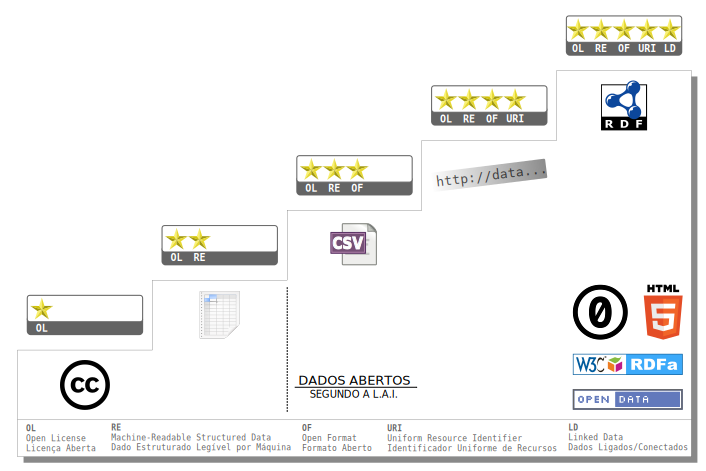
\includegraphics[width=1.0\textwidth]{imagens/open_data_stars.png}
  \caption{Classificação dos dados abertos segundo a escala de 5 estrelas de Berners-Lee}
  \label{fig:LABEL_FIG_OPEN_STARS}
\end{figure}

\begin{itemize}

\item \textbf{1 estrela}: Disponibilizar o dado na web (em qualquer formato) sob uma licença aberta.

\item \textbf{2 estrelas}: Tornar o dado estruturado (exemplo: uma planilha no Excel ao invés de uma imagem digitalizada de uma tabela).

\item \textbf{3 estrelas}: Tornar o dado disponível em um formato aberto, não-proprietário (exemplo: CSV ao invés de XLS, do Excel).

\item \textbf{4 estrelas}: Utilizar URIs para denotar os dados, para que as pessoas possam referenciá-los.

\item \textbf{5 estrelas}: Conectar os dados a outros datasets a fim de fornecer um contexto (\textit{linked data}\footnote{O conceito de linked data (dados ligados entre si) é um conjunto de práticas introduzidas por Tim Berners-Lee, com função de publicar e estruturar dados na Web, agregando valor semântico aos dados.}).

\end{itemize}



{\large Dados Abertos Governamentais}

Apesar de as definições de dados abertos serem gerais o suficiente para qualquer contexto, foram elaborados princípios mais específicos como referência para dados abertos governamentais, isto é, dados abertos sob posse de um governo\cite{REF_OGD_PRINCIPLES}. Um grupo de trabalho de 30 pessoas situado na Califórnia, Estados Unidos, o \textit{Open Government Working Group}, chegou a um consenso sobre os seguintes princípios:

\begin{enumerate}
\item \textbf{Completos}. Todos os dados públicos são disponibilizados. Dados são informações eletronicamente gravadas, incluindo, mas não se limitando a, documentos, bancos de dados, transcrições e gravações audiovisuais. Dados públicos são dados que não estão sujeitos a limitações válidas de privacidade, segurança ou controle de acesso, reguladas por estatutos.

\item \textbf{Primários}. Os dados são publicados na forma coletada na fonte, com a mais fina granularidade possível, e não de forma agregada ou transformada.

\item \textbf{Atuais}. Os dados são disponibilizados o quão rapidamente seja necessário para preservar o seu valor.

\item \textbf{Acessíveis}. Os dados são disponibilizados para o público mais amplo possível e para os propósitos mais variados possíveis.

\item \textbf{Processáveis por máquina}. Os dados são razoavelmente estruturados para possibilitar o seu processamento automatizado.

\item \textbf{Acesso não discriminatório}. Os dados estão disponíveis a todos, sem que seja necessária identificação ou registro.

\item \textbf{Formatos não proprietários}. Os dados estão disponíveis em um formato sobre o qual nenhum ente tenha controle exclusivo.

\item \textbf{Livres de licenças}. Os dados não estão sujeitos a regulações de direitos autorais, marcas, patentes ou segredo industrial. Restrições razoáveis de privacidade, segurança e controle de acesso podem ser permitidas na forma regulada por estatutos.
\end{enumerate}

Uma vez tendo em mãos esses dados, há diversos possíveis usos dos mesmos refletindo em diferentes aspectos da sociedade. Os DAGs trazem impacto direto na política e são causadores de um grande movimento de \textit{accountability}, isto é, uma responsabilidade aos governos a partir das informações oriundas desses dados. Dessa forma, podemos enxergar que quanto maior o acesso a essas informações, maiores as chances de que a sociedade acompanhe as iniciativas do poder público e as fiscalize, eventualmente contribuindo para a melhora do serviço público.

Outro grande reflexo dos DAGs é em termos de mercado. A partir da mineração dos dados abertos, que vêm como dados brutos, é possível extrair novas informações e agregá-las na forma de  produtos e serviços de valor para os usuários. Tem-se então a criação de novos negócios a partir dos DAGs. Alguns dos possíveis modelos de negócios a partir de DAGs e seus impactos na economia foram estudados por \cite{REF_MONO_BUUS}. 

\chapter{Rio Bus}\label{chp:CAP_RIOBUS}

Uma aplicação real que faz uso dos DAGs e que serviu como plataforma para este trabalho é o \textbf{Rio Bus}\cite{riobus_sc}, projeto do qual faço parte. Criado por alunos do curso de Bacharelado em Ciência da Computação da UFRJ, o Rio Bus surgiu em 2014 como um aplicativo para visualizar em um mapa a posição em tempo real dos ônibus municipais do Rio de Janeiro, utilizando os recém-lançados dados abertos de mobilidade oferecidos pela Prefeitura do Rio de Janeiro. Com esse serviço, o cidadão pode estimar o quanto vai demorar para seu ônibus chegar e, assim, se planejar melhor.


\begin{figure}
  \centering
  \includegraphics[width=0.5\textwidth]{imagens/riobus.png}
  \label{fig:LABEL_FIG_RIOBUS}
\end{figure}


Lançado gratuitamente e como um projeto de \textit{open-source}, o Rio Bus logo conseguiu vários colaboradores, usuários do aplicativo, dentro da UFRJ, haja vista a grande demanda por transporte público no campus da Universidade. A solução foi então disponibilizada em diferentes plataformas - um \textit{website}, disponível em \cite{REF_RIOBUS_WEB}, para acesso pelo computador ou dispositivos móveis, e dois aplicativos para \textit{smartphones}, um para o sistema operacional \textit{Android}, do Google, disponível em \cite{REF_RIOBUS_ANDROID}, e outro para \textit{iOS}, da Apple, disponível em \cite{REF_RIOBUS_IOS}.

Pouco tempo após seu lançamento, o aplicativo ganhou uma grande repercussão e serviu como ferramenta para muitos cidadãos durante a greve dos ônibus, em março de 2014. Durante a paralisação, na qual cerca de 80\% da frota de ônibus do município não saiu da garagem das empresas, muitos usuários fizeram uso do aplicativo para saber se suas linhas de ônibus estavam circulando e acompanhar onde estavam os coletivos. Esse evento não só serviu como a tração que o Rio Bus precisava para seu sucesso, como também foi um grande \textit{insight} de que coletar os dados que vinham sobre os ônibus poderia servir para uma análise do funcionamento do serviço. Esses estudos não só ajudaram a melhor compreender o serviço dos ônibus no Rio e suas falhas, como também podem ter importância especial durante períodos atípicos como paralisações, alterações no sistema, grandes eventos e ocorrências de trânsito na cidade.


\section{Base de dados}

\subsection{Origem}

Para popular a base de dados do Rio Bus, são utilizados os dados dos ônibus fornecidos pelo Data.rio\cite{data.rio}, o portal de dados abertos da Prefeitura do Rio de Janeiro. O Data.rio disponibiliza um total de 1200\footnote{Número de conjuntos de dados disponíveis em http://data.rio/ em 6 de julho de 2016} conjuntos de dados (\textit{datasets}) que estão classificados em 13 grupos - entre eles, Urbanismo, Administração Pública, Impostos e Transporte e Mobilidade, que foi o grupo utilizado.

Dentre os dados de Transporte e Mobilidade, há 23 conjuntos de dados que incluem informações sobre ônibus, trens, metrô, barcas e bicicletários do Rio de Janeiro. Estamos interessados em 3 desses \textit{datasets}: GPS dos ônibus, Pontos de parada das linhas do ônibus e Pontos dos trajetos das linhas de ônibus. Esses dados são fornecidos em parceria da Prefeitura do Rio com a FETRANSPOR (Federação das Empresas de Transporte de Passageiros do Estado do Rio de Janeiro).


\subsection{Formatos}

São utilizados diferentes formatos para acesso aos dados do Data.rio. Os dados dos pontos de parada e pontos de trajeto das linhas dos ônibus são dados tipicamente estáticos - isto é, não costumam sofrer alterações frequentes - e são disponibilizados em uma planilha em formato CSV (Comma-separated values). Eles são atualizados com baixa frequência na base de dados do Rio Bus.

Já os dados de GPS dos ônibus, como são atualizados diversas vezes por minuto, podem ser acessados através de uma API (Application Programming Interface) que retorna um objeto JSON (JavaScript Object Notation) contendo os dados de cada ônibus naquele instante. Esses dados são coletados com alta frequência para popular a base de dados do Rio Bus, formando assim uma coleção histórica dos dados. Um exemplo de como se parece essa coleção está na tabela \ref{table:collection_bus}, que mostra um trecho dos registros de um ônibus da linha 325 no dia 09/07/2015.

\begin{table}[]
\centering
\caption{Exemplo da coleção histórica de um ônibus}
\label{table:collection_bus}
\begin{tabular}{|p{2.5cm}|c|c|c|c|c|c|}
\hline
\multicolumn{7}{|c|}{\textbf{Trecho da coleção histórica do ônibus B28518 da linha 325}} \\
\hline
\textbf{Data/hora} & \textbf{Ordem} & \textbf{Linha} & \textbf{Lat.} & \textbf{Long.} & \textbf{Veloc
.} & \textbf{Direção} \\ \hline
09/07/2015 23:19:05 & B28518 & 325 & -22.815200 & -43.188300 & 41 & 306\\\hline
09/07/2015 23:20:18 & B28518 & 325 & -22.815700 & -43.188100 & 20 & 165\\\hline
09/07/2015 23:21:35 & B28518 & 325 & -22.815700 & -43.188000 & 37 & 150\\\hline
\end{tabular}
\end{table}


\subsection{Armazenamento}

Como o volume de dados proveniente da atualização dos ônibus é muito grande, as APIs do Data.rio fornecem apenas os dados do instante atual. Para que pudéssemos ter acesso aos dados de períodos passados, utilizamos a infraestrutura do \textit{back-end} do Rio Bus para armazenar esses dados, que ultrapassam 9 milhões de novos registros por dia.

Para isso, temos um serviço que executa indefinidamente que faz a leitura dos dados do Data.rio e os salva num banco de dados próprio. Na implementação atual, os dados são salvos em dois lugares: numa coleção do MongoDB, um banco de dados não-relacional open-source instalado localmente, e no Google BigQuery, um serviço de cloud para armazenamento e análise de dados em larga escala (\textit{Big Data}), como é o nosso caso.

Para os propósitos deste trabalho, daremos preferência ao banco de dados MongoDB\cite{REF_MONGODB} para executar as consultas. Ainda que a implementação das consultas nele seja mais difícil - o Google BigQuery\cite{REF_BIGQUERY} suporta consultas com SQL - a decisão leva em conta o acesso à informação - o BigQuery é um serviço pago, remoto e de código fechado, enquanto o MongoDB é uma aplicação que pode ser executada localmente, sem custos e que possui o código aberto, de acordo com os princípios deste projeto.


\chapter{A análise dos dados}\label{chp:CAP_ANALISE}

O escopo inicial deste trabalho propôs 4 diferentes análises:

\begin{enumerate}

\item \textbf{Frequência da linha}: calcula qual foi a frequência e tempo médio de espera por ônibus de uma linha. Reflete quanto tempo um usuário costuma esperar, em média, até que passe seu ônibus, em cada horário do dia. Pode ser usada para comparação com a frequência informada por cada companhia e para o próprio usuário poder estimar o tempo que irá aguardar até embarcar.

\item \textbf{Concentração da frota}: mostra onde os ônibus estiveram nas últimas 24 horas, mostrando quais regiões possuem maior concentração de ônibus e quais sequer possuem linhas de ônibus.

\item \textbf{Quantidade de ônibus por linha e hora}: similar ao estudo anterior, porém  mostra quantos carros de cada linha estavam circulando em cada horário do dia. Pode ser comparada com a quantidade de veículos determinada nas concessões da Prefeitura às companhias de ônibus.

\item \textbf{Atualização do GPS}: uma meta-análise dos DAGs para monitorar a qualidade do monitoramento dos ônibus em relação à atualização dos dados. Pode servir pra mostrar quais companhias não estão transmitindo os dados de sua frota e, portanto, descumprindo seu contrato com a Prefeitura.

\end{enumerate}

Foram desenvolvidos os estudos 1 e 2, que serão descritos em detalhes a seguir.


\renewcommand{\labelenumii}{\theenumii}
\renewcommand{\theenumii}{\theenumi.\arabic{enumii}.}

\section{Frequência dos ônibus}

Este estudo tem como objetivo analisar a frequência dos ônibus de uma linha, de maneira que o resultado final reflita qual o tempo médio de espera por um ônibus daquela linha em um certo horário do dia. Tal informação não é oferecida pelos DAGs utilizados e, apesar de algumas companhias de ônibus divulgarem uma frequência oficial de suas linhas, muitas vezes estas não são cumpridas ou, na prática, são afetadas por outros fatores, como o trânsito.


\subsection{Dados utilizados}

As estatísticas são obtidas a partir de uma amostra dos registros de localização dos ônibus em um período de 24 horas. Como as linhas possuem diferentes características, cada linha foi analisada individualmente e os dados médios serão agrupados por hora.

Também são usados para compreensão desses dados a informação geolocalizada dos pontos de parada da linha.


\subsection{O algoritmo}

Calcularemos o intervalo de tempo entre cada ônibus da linha em diversos pontos ao longo do itinerário. Considere disponíveis as variáveis e funções abaixo:

\begin{itemize}
    \item $L$: a linha a ser analisada (ex.: $485$);
    \item $D$: a data a ser analisada (ex: $08/10/2015$);
    \item $stops(L)$: função que retorna o conjunto de pontos de parada geolocalizados da linha $L$;
    \item $history(L,D)$ a função que retorna os registros geolocalizados dos ônibus da linha $L$ na data $D$;
    \item $matches(R,p)$ a função que retorna o subconjunto dos registros $R$ próximos a um ponto de parada $p$.
\end{itemize}

O algoritmo desenvolvido é descrito a seguir.

\begin{enumerate}

\item Obter $P = stops(L)$ e $R = history(L,D)$.
%\item Obter as informações dos pontos de parada da linha e as posições dos ônibus da linha selecionada, para o dia analisado.

\item Para cada ponto $p_i$ de $P$: 

    \begin{enumerate}
        \item Obter $M_i = matches(R,p_i)$, isto é, os registros dos ônibus que passaram pelo ponto de parada $p_i$.
        
        \item Ordenar $M_i$ pelo horário dos registros de forma ascendente.\footnote{Obtém-se ao final da ordenação a sequência de cada ônibus que passou por aquele ponto ao longo do dia - assim como teria, por exemplo, um fiscal da companhia de ônibus, cuja função é anotar os horários em que cada ônibus da companhia passou por ali.}
        
        \item Eliminar de $M_i$ registros de um mesmo ônibus com horários próximos, a fim de evitar que ele seja contado mais de uma vez.\footnote{Caso o ônibus encontre-se parado durante muito tempo no ponto ou próximo a ele, pode haver mais de um registro, cujos cruzamentos duplicados devem ser descartados.}
        
        \item Dividir os cruzamentos de $M_i$ em 24 subconjuntos $M_{ij}$ de acordo com a hora de cada registro ao longo do dia.
        
        \item Para cada conjunto $M_{ij}$, $0 \leq j < 24$, calcular o intervalo de tempo entre cada registro do conjunto e a média $I_{ij}$ dos intervalos.
        
    \end{enumerate}
    
\item Para cada hora do dia, $0 \leq j < 24$, calcular a média entre todos os pontos $i$ dos intervalos $I_{ij}$. 

\end{enumerate}

Ao fim do algoritmo, obtém-se um conjunto com 24 médias, representando o intervalo médio - ou seja, a frequência - dos ônibus daquela linha em cada hora do dia.

O motivo de a frequência dos ônibus ser analisada por hora é devido ao próprio modelo de funcionamento das linhas, que possui frequências variáveis de acordo com a demanda de cada horário.

Através do algoritmo mostrado, também é possível calcular qual foi o tempo de retorno do ônibus, indicando o tempo total de viagem na linha (ida + volta). Para isso, basta calcular o tempo entre duas ocorrências do mesmo ônibus no mesmo ponto e com o mesmo sentido - ou seja, o tempo que o ônibus levou desde que passou ali até percorrer a linha toda e passar ali de novo.


\subsection{Implementação}

O algoritmo foi implementado em Node.js, que é um ambiente de desenvolvimento em JavaScript\cite{REF_JAVASCRIPT}\cite{REF_NODEJS}. Essa escolha foi feita principalmente devido à velocidade do desenvolvimento e por ser uma boa linguagem de prototipagem\cite{REF_NODEJS_PROTOTYPING} e possui um excelente suporte ao MongoDB, banco de dados utilizado.

Foi desenvolvido um programa que faz a conexão com o banco de dados, já populado, executando o algoritmo acima e exportando os dados calculados para um arquivo JSON. 

Também foi criada uma página HTML\cite{REF_HTML} que usa JavaScript para ler os dados do arquivo JSON e plotá-los num gráfico de barras, a fim de facilitar a visualização dos dados de hora em hora ao longo do dia analisado.


\subsection{Resultados observados}

Foi utilizado como exemplo do estudo o histórico de julho de 2015 da linha 324, que faz o percurso Ribeira (Ilha do Governador) x Candelária (Centro). Segundo o site da empresa que controla essa linha, a Viação Ideal, a frequência média oficial é de 9 minutos entre cada ônibus\cite{ideal_324}.

Na figura \ref{fig:LABEL_FIG_ANALISE_FREQ_324}, os dados analisados são de um dia útil. Podemos observar durante a manhã desse dia que o tempo médio de espera por um ônibus dessa linha fica em torno de 20 minutos, com pequenos aumentos chegando a 25 minutos para quem aguardava um ônibus entre as 8 e 10 horas, período com reflexos do horário do rush. Já na faixa das 12 horas, nenhuma média foi calculada, pois não houve frequência suficiente de ônibus nos pontos analisados para que o algoritmo pudesse calcular uma média. Durante o começo da tarde, vemos um grande aumento no tempo de espera, provavelmente causado pelo mesmo motivo que causou a falta de dados no período das 12 horas, que foi normalizando nas horas seguintes até que aumentou de novo a partir das 19 horas.

Uma comparação da análise desse dia pode ser feita com a da figura \ref{fig:LABEL_FIG_ANALISE_FREQ_324_DOMINGO}, com os dados da mesma linha porém em um domingo. Duas observações podem ser feitas imediatamente: a média de espera é maior, pois aos finais de semana há menos ônibus circulando e também o tempo de espera é bem mais constante, visto que num domingo não há trânsito causando atrasos na circulação dos ônibus.

Com uma base de dados maior, é possível fazer tais comparações entre datas mais relevantes, a fim de observar os reflexos na frequência dos ônibus causados por eventos, interdições, desvios e outros fatores. Também é possível agregar dados analisados em intervalos maiores.

\begin{figure}
  \centering
  \includegraphics[width=1.0\textwidth]{imagens/grafico_freq.png}
  \caption{Análise mostra o tempo médio de espera por um ônibus da linha 324 num dia útil em julho de 2015.}
  \label{fig:LABEL_FIG_ANALISE_FREQ_324}
\end{figure}

\begin{figure}
  \centering
  \includegraphics[width=1.0\textwidth]{imagens/grafico_freq_dom.png}
  \caption{Análise mostra o tempo médio de espera por um ônibus da linha 324 num domingo em julho de 2015.}
  \label{fig:LABEL_FIG_ANALISE_FREQ_324_DOMINGO}
\end{figure}

Apesar de o algoritmo ser relativamente simples, houve uma grande dificuldade na filtragem dos registros duplicados. Ao observar que os resultados da execução com uma certa linha estavam apontando um resultado surpreendentemente bom, notamos que existe um cenário específico em que os ônibus são erroneamente identificados cruzando um ponto de parada.

Foi comparada a execução do algoritmo em diferentes linhas com resultados similares. Concluiu-se que estava sendo computado um falso positivo dos ônibus que cruzavam um ponto de parada no sentido contrário ao esperado. Logo, observou-se que isso era um cenário recorrente nas linhas em que o itinerário de ida era similar ao itinerário de volta, como quando uma linha passa na mesma rua nos dois sentidos. Nesse caso, os pontos de parada da ida são muito próximos aos pontos da volta - às vezes com pouquíssimos metros de distância, apenas em lados opostos da rua.

O algoritmo que calcula o cruzamento de um ônibus com um ponto de parada através de seu raio de proximidade acabava identificando um falso positivo nesses casos. Visando contornar esse problema, foi necessário implementar essa diferenciação do sentido por conta própria.

A fim de identificar se um ônibus está no seu itinerário de ida ou de volta, foi elaborado um algoritmo que identifica qual o sentido comparando a posição atual do ônibus com a sua posição nos últimos registros. Considerando que conhecemos o itinerário da linha, comparamos o histórico das últimas $n$ posições conhecidas do ônibus, guardadas na memória, com o itinerário dos dois sentidos, analisando se o trajeto pertence ao conjunto da ida ou da volta.

Uma vez conhecido o sentido atual, esse dado é salvo junto ao registro do ônibus para que possa ser utilizado posteriormente. Para identificar se um determinado ônibus realmente passou por um ponto de parada, verificamos se o sentido registrado naquele instante condiz com o sentido do ponto. Caso sejam diferentes, esse registro é descartado, eliminando o falso positivo.

\section{Concentração da frota}

A proposta deste estudo é evidenciar, através de um mapa de calor, onde estão concentrados os ônibus pela cidade ao longo de um dia. Pode ser usada como ferramenta para o planejamento de novas linhas e redistribuição das atuais. 

Apesar de ser difícil extrair conclusões apenas com este mapa, ele pode servir como uma ferramenta visual para observar em que vias e regiões da cidade estão concentrados os ônibus. Um exemplo é a figura \ref{fig:LABEL_FIG_ANALISE_CONCENTRACAO_CIDADE}, que traz uma visão geral da cidade do Rio de Janeiro.

\begin{figure}
  \centering
  \includegraphics[width=1.0\textwidth]{imagens/heat_map1.png}
  \caption{Vista geral da cidade mostra uma grande concentração de ônibus nas regiões centrais. (Outubro de 2015)}
  \label{fig:LABEL_FIG_ANALISE_CONCENTRACAO_CIDADE}
\end{figure}


\subsection{Implementação}

Por ser uma análise mais simples, o esforço maior desta análise foi na parte da apresentação dos dados, ao invés da extração dos mesmos. 

Para extrair os dados, foi feita uma consulta no banco de dados por todos os registros geolocalizados em uma data específica. Como extrair e plotar esses dados diretamente seria muito demorado - há mais de 15 milhões de registros por dia - optamos por reduzir manualmente a precisão desses dados, agrupando registros muito próximos.

Para agrupar essas amostras, limitamos na nossa consulta a precisão dos campos de latitude e longitude de cada registro, utilizando uma precisão máxima de 4 casas decimais ao invés de 6. Só isso já reduz nosso número de amostras em cerca de 35 vezes, para cerca de 420.000 amostras, ainda mantendo uma boa precisão visual dos dados. 

Finalmente, a fim de descobrir quantos ônibus estavam em cada coordenada, foi utilizada a quantidade de registros naquela posição, contando apenas veículos distintos (cada ônibus é identificado por um número de ordem). Temos então como saída uma lista de coordenadas e suas respectivas quantidades de ônibus. 

Cada coordenada é plotada no gráfico através de uma escala de cores que representa a densidade de ônibus naquela região\cite{heatmap}. Como resultado, temos cores entre o azul escuro, que representa uma baixa densidade de ônibus na região, e o vermelho, que representa uma alta densidade. As escalas de cores foram normalizadas entre os estudos para preservar facilitar a comparação entre diferentes mapas.

Para a visualização desses dados, foi elaborada uma página que renderiza um mapa interativo, no qual é possível alterar a região de estudo e observar com maior precisão os resultados, permitindo focar em bairros ou ruas específicas. Quando duas amostras são comparadas, é possível visualizá-las lado-a-lado, atualizando simultaneamente conforme o mapa é movimentado pelo usuário.


\subsection{Resultados observados}

O mapa de calor se torna ainda mais útil quando são comparados dados de diferentes períodos, a fim de analisar como mudou a distribuição dos ônibus ao longo do tempo.

Uma das comparações feitas foi entre dados de dois anos consecutivos, 2015 e 2016. Foram analisados dados do mesmo dia, 8 de julho, um dia útil, nos dois anos. A comparação entre esses anos é especialmente relevante pois, desde o final de 2015 até a data atual, ocorrem grandes mudanças nas linhas de ônibus do Rio de Janeiro, em especial devido ao plano de racionalização das linhas da Zona Sul\cite{noticia_racionalizacao}. Além disso, devido a grandes obras pela cidade, houve diversas interdições no trajeto das linhas, a construção de novas vias e implantação de novos corredores exclusivos de ônibus.

Na figura \ref{fig:LABEL_FIG_ANALISE_RACIONALIZACAO}, é possível visualizar essa comparação e observar uma enorme diminuição dos ônibus nos bairros da Zona Sul próximos à Lagoa Rodrigo de Freitas. 

\begin{figure}
  \centering
  \includegraphics[width=1.0\textwidth]{imagens/heat_map_zs201516.png}
  \caption{Comparação da quantidade de ônibus na Zona Sul em dois anos consecutivos. Em 2016, observa-se a redução em virtude da racionalização das linhas de ônibus.}
  \label{fig:LABEL_FIG_ANALISE_RACIONALIZACAO}
\end{figure}


No Centro da cidade, observa-se através da figura \ref{fig:LABEL_FIG_ANALISE_CONCENTRACAO_CENTRO} que as principais vias da região concentram praticamente toda a circulação dos ônibus, enquanto vias transversais não possuem quase nenhum tráfego desse tipo.

\begin{figure}
  \centering
  \includegraphics[width=0.9\textwidth]{imagens/heat_map2.png}
  \caption{No Centro, concentração alta nas vias principais e baixa nas transversais. (Outubro de 2015)}
  \label{fig:LABEL_FIG_ANALISE_CONCENTRACAO_CENTRO}
\end{figure}

% \begin{figure}
%   \centering
%   \includegraphics[width=1.0\textwidth]{imagens/heat_map3.png}
%   \caption{Enorme concentração em um único trecho em Campo Grande. (Outubro de 2015)}
%   \label{fig:LABEL_FIG_ANALISE_CONCENTRACAO_3}
% \end{figure}

\chapter{Conclusões}\label{chp:CAP_CONCLUSOES}

Com os estudos realizados, foi possível construir mais uma prova de como os DAGs podem ser úteis à sociedade. As duas análises desenvolvidas são exemplos de como esse tipo de ferramenta pode ser usada para ampliar a transparência de serviços como o transporte público. Porém, ao mesmo tempo que temos que agradecer pela disponibilidade desses dados públicos, ainda há muito o que se reivindicar no que diz respeito à qualidade e à cobertura dos dados fornecidos, visto que existem diversos problemas que foram observados durante os estudos.

Foram identificadas algumas dificuldades em relação à confiabilidade dos dados coletados, uma vez que a base de dados que utilizamos da Prefeitura não possui informações completas sobre as linhas. Além disso, também há uma enorme quantidade de dados desatualizados, o que impede a execução correta dos algoritmos para a análise, causando a disponibilização de informações incorretas à população que utiliza serviços como o Rio Bus, por exemplo. 

Há alguns exemplos de como tais problemas afetaram este estudo:

\begin{itemize}
    \item Diversas linhas em circulação não possuem informações sobre seu itinerário, um dos dados oferecidos pelo Data.rio, enquanto diversas outras possuem itinerários desatualizados. Sem esses dados não há uma referência para a comparação das linhas através de algoritmos.
    \item Assim como o itinerário, faltam informações sobre os pontos de parada ou estão desatualizadas em diversas linhas, o que impede a execução da análise da frequência dos ônibus ou causa resultados não confiáveis.
    \item Mudanças que não existiam ou que ocorriam em menor escala nas linhas de ônibus no Rio de Janeiro ocorreram com grande frequência no último ano, dificultando os estudos, tais como a mudança de 180 linhas que passam pelo Centro do Rio em maio de 2016\cite{noticia_centro_mudancas} e o plano de racionalização das linhas, que reduziu de 123 para 45 as linhas que passam pela Zona Sul do Rio\cite{noticia_racionalizacao}.
    \item Não é informado pelos DAGs qual o sentido do ônibus em cada instante, o que acaba tendo de ser calculado manualmente para que essa informação seja usada para calcular com maior precisão o tempo de espera em cada parada.
    \item Há falhas frequentes na transmissão dos dados de posição dos ônibus, com linhas ou até mesmo consórcios inteiros\footnote{As empresas de ônibus que operam no Rio de Janeiro são agrupadas em 4 diferentes consórcios - Internorte, Intersul, Transcarioca e Santa Cruz - que operam em diferentes áreas da cidade. Fonte: Rio Ônibus (http://www.rioonibus.com/rio-onibus/consorcios-e-empresas/). Acessado em outubro de 2016.} que "desaparecem" \textit{} durante períodos, conforme observado em 2015, quando o consórcio Internorte ficou meses sem transmitir dados de todas as suas linhas.
    \item A própria API do Data.rio possui problemas, ocasionalmente ficando indisponível sem nenhum aviso prévio e alterando o contrato de seus serviços sem a documentação apropriada, o que causou interrupções e falhas na coleta dos dados.
\end{itemize}

Devido aos problemas relatados anteriormente, a complexidade do trabalho se tornou maior, pois foi necessário elaborar soluções além do escopo inicial para que se obtivesse maior confiabilidade dos resultados, causando interrupções no desenvolvimento dos estudos e criando limitações nas linhas que poderiam ser analisadas.

Outros problemas encontrados foram em relação ao armazenamento dos dados e à complexidade de processamento dos mesmos. Com a enorme quantidade de dados produzida a cada dia, armazenar dados históricos localmente tornou-se um problema em diversos aspectos, como o uso de espaço em disco, a disponibilidade de servidores capazes de colher esses dados ininterruptamente e a complexidade de processamento dos dados. Embora a infraestrutura do Rio Bus e seus serviços, de código aberto, tenham ajudado nesse aspecto, ainda dependíamos de serviços externos como o Google BigQuery para consultar esses dados históricos, o que gerou custos e mais um nível de dependência.

Quanto à complexidade de processamento, processar dados de longos períodos ou de muitas linhas simultaneamente foi bastante demorado. Por este motivo, o estudo da frequência dos ônibus no escopo deste trabalho limitou-se a apenas uma linha e a um dia por vez, embora pudesse ser otimizado para análises mais elaboradas.

Apesar de todos os desafios encontrados, a ferramenta desenvolvida serviu como uma prova de conceito de que é possível utilizar os DAGs como instrumento para a fiscalização do serviço de transporte no Rio. Com as análises desenvolvidas, foi possível observar que o serviço prestado deixa muito a desejar, e como as mudanças nos planos de transporte da cidade afetam a disponibilidade das linhas.

Ainda que o objetivo inicial deste trabalho propusesse uma facilidade maior de acesso às estatísticas coletadas, todos os algoritmos desenvolvidos durante os estudos foram disponibilizados no GitHub\footnote{GitHub: site que permite que as pessoas hospedem e compartilhem códigos versionados, e concentra o maior número de projetos open-source disponíveis, com uma enorme comunidade de contribuidores. (https://github.com)}, podendo ser executados, modificados ou redistribuídos por qualquer um, assim como o código do Rio Bus, que serviu como uma útil ferramenta para a coleta dos dados abertos.


\section{Trabalhos futuros}

Apesar de o projeto ter sofrido limitações devido à base de dados utilizada, suas propostas e algoritmos podem ser facilmente reproduzidos em outras bases de dados, servindo a diferentes propósitos e podendo ser facilmente estendidos e aprimorados para outros meios de transporte.

Substituindo a base de dados utilizada, é possível reproduzir os estudos em diferentes cidades que disponibilizam os dados dos ônibus como DAGs e até mesmo em diferentes meios de transportes. Embora o estudo tenha sido pensado com o funcionamento dos ônibus públicos, as mesmas análises podem ser aplicadas a frotas de ônibus privados, táxis, carros ou caminhões. Um serviço de monitoramento e de relatórios gerenciais de frota pode ser aplicado para fins comerciais e oferecido a cooperativas, transportadoras e empresas de ônibus, como é apontado por \cite{REF_MONO_BUUS}.

Com a infraestrutura adequada, o cálculo das análises também pode ser automatizado para que, por exemplo, a frequência de cada linha seja calculada ao final de cada dia. Dessa maneira, os estudos desenvolvidos podem se tornar ainda mais completos, e os resultados podem ser disponibilizados em uma página abrangendo todas as linhas de ônibus.

O algoritmo de análise da frequência também pode ser explorado com outras abordagens de implementação, como, por exemplo, aprimorando o paralelismo do algoritmo. Tal mudança melhoraria o desempenho de processamento, algo especialmente importante caso se queira analisar o conjunto de todas as linhas de maneira eficiente.

Ainda visando uma ferramenta pública para a consulta desses dados, pode ser criado um repositório contendo as diferentes análises propostas, para que qualquer cidadão possa consultá-las, mesmo sem possuir conhecimento técnico.

\pagebreak

%%%%%%%%%%%%%%%%%%%%%%%%%%%%%%%%%%%%%%%%%%%%%%%%%%%%%%%%%%%%
% B I B L I O G R A F I A
%%%%%%%%%%%%%%%%%%%%%%%%%%%%%%%%%%%%%%%%%%%%%%%%%%%%%%%%%%%%
\makebibspage{abnt}{elementos-postextuais/referencias}


\end{document}